\section{Corrientes relacionadas}
%\observacion{Agregar partes de simulación, ver ./simulacion.tex}
%\observacion{Agregar ECA}

Los juegos serios son el solapamiento de tres corrientes, los videojuegos, las
técnicas de enseñanza y la simulación\cite{education:games}, tal y
como se observa en la figura~\ref{fig:corrientes_relacionadas}. 

\begin{figure}[ht]
\centering
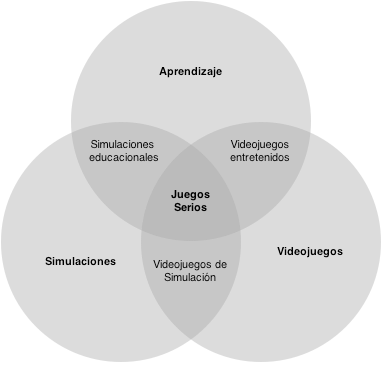
\includegraphics[scale=0.7]{juegos_serios/corrientes_paralelas.png}
\caption{Ubicación de los juegos serios entre los videojuegos, la simulación y
    la educación}
\label{fig:corrientes_relacionadas}
\end{figure}

Cuando se utilizan aspectos de videojuegos con simulaciones, se obtienen videojuegos
cuyo objetivo es entretener mientras son similares a la realidad, dentro de esta
categoría podemos encontrar juegos como \emph{Gran Turismo}; si mezclamos
factores relacionados al aprendizaje y a las simulaciones se obtienen
simulaciones sin interacción con el usuario que buscan mostrar o enseñar como se
comportan distintos fenómenos físicos, sociales, etc.

Un simulación educativa se diferencia de un juego serio en que este último hace uso 
de las características y tecnologías de un videojuego para enseñar algo específico. Los 
\emph{Edutainment} pueden ser vistos como los predecesores de los juegos
serios, los mismos son descritos en~\ref{sec:edutainment}.

%\observacion{Que hace que sea un juego serio y no una SE}

Usualmente un videojuego tiene un conjunto de reglas que deben ser cumplidas para 
que se considere que una partida fue jugada de manera correcta, lo que se traduce 
en un buen desempeño del jugador, estas reglas suelen ser manejadas
por un motor de reglas que se encarga de determinar el cumplimiento o no de las mismas.

\subsection{Simulaciones}

La simulación se define como el proceso de diseñar un modelo de un sistema real
y, llevar a cabo experimentos con este modelo, con el fin o bien de entender el
comportamiento del sistema o de la evaluación de distintas estrategias para la
operación del sistema\cite{ingalls2008introduction}. 

Aunque un juego serio y una simulación pueden parecer muy similares, se
diferencian en que, si bien muchos videojuegos incluyen una simulación, una
simulación no utiliza características típicas de los videojuegos como la
fantasía, puntuación, etc\cite{sg:aoverview}.

La simulación en el ámbito de la educación evolucionó desde simples motores de
reglas hasta complejos entornos. La simulación demostró ser una herramienta muy
útil en el ámbito laboral\cite{mariluz:seiousgames}, pues enseña al usuario a
encarar situaciones muy difíciles de representar en entornos completamente
controlados y provee mecanismos para comprobar la efectividad de la herramienta. 

Actualmente la simulación se utiliza más en el ámbito empresarial pues las
empresas son las más necesitadas de innovar en el ámbito de la enseñanza. Un
ejemplo de esta necesidad se da, por ejemplo, en el entrenamiento de nuevos
vendedores, es muy difícil enseñar a un vendedor como debe vender los productos
con un pizarrón y/o una presentación, en cambio la simulación permite que el
mismo pueda probar cosas nuevas y experiencias de sus compañeros (o instructor),
convirtiendo así el aprendizaje en colectivo\cite{mariluz:seiousgames}.

Existen dos tipos de simulaciones, en primer lugar están las experimentales que
ponen al estudiante en el lugar de un profesional y requieren que el mismo tome
decisiones para alcanzar los objetivos y en segundo lugar están las simbólicas
que buscan que el estudiante deduzca eventos, principios y mejores
prácticas\cite{charsky:2010}. 

%La simulación se compone de tres elementos principales, entidades (que son
%objetos de la vida real), acciones (que son provocadas por las entidades) y
%eventos (que son el resultado de una acción). A continuación son detalladas 
%cada una de estas partes.

%\begin{itemize}
%\item \textbf{Entidades:} una entidad es cualquier objeto o componente en el 
%sistema que requiera la representación explícita en el modelo\cite{banks2000dm}. 
%Las entidades tienen atributos. Los atributos son las características de una 
%determinada entidad que son exclusivos de esa entidad.

%\item \textbf{Acciones:} las entidades se comunican a través de acciones, las cuales 
%pueden tener diversos orígenes, siempre una entidad inicia una acción. Las acciones 
%provocan cambios en el ambiente y provocan eventos. Las acciones no solo las
%realiza el usuario, sino cualquier entidad.

%\item \textbf{Eventos:} los eventos son ocurrencias instantáneas que cambian el 
%estado de un sistema\cite{banks2000dm}, cada acción que se realiza provoca otra 
%acción, y los eventos son el mecanismo que tiene una entidad para ser notificada 
%de las acciones de otras entidades.

%\end{itemize}


%\subsection{Diferencia entre juegos serios, simulaciones y los Edutainment}
%\observacion{Por que esta comparación? Énfasis en simulaciones educativas}

%Estos tres entornos virtuales altamente interactivos, poseen posibilidades y
%fines distintos, pueden parecer similares pero poseen las siguientes
%diferencias\cite{education:games}:

%\begin{itemize}
%\item \textbf{Simulaciones educativas}: utilizan escenarios rigurosamente
%    estructurados con un conjunto altamente refinado de normas, retos y
%    estrategias que son cuidadosamente diseñados para desarrollar las
%    competencias específicas que se pueden transferir directamente al mundo
%    real.
%\item \textbf{Videojuegos:} son actividades atractivas y divertidas que
%    habitualmente se utilizan exclusivamente para el entrenamiento pero también
%    permiten una exposición con un conjunto determinado de herramientas,
%    argumentos o ideas. Todas las partidas se juegan en un mundo estructurado
%    por normas específicas, mecanismos de retroalimentación, y las herramientas
%    necesarias, aunque no están tan definidas como en las simulaciones.

%\item \textbf{Edutainment:} son aplicaciones educativas cuyo principal propósito
%    es el de entretener, y el aprendizajes es un añadido. Los
%    \emph{edutainment}, se centran en la motivación externa.
%\end{itemize}


\subsection{Acciones condicionadas por eventos}
\label{sec:eca}

Un evento es la ocurrencia de un hecho en particular, y es identificado por un
nombre y un conjunto de parámetros. Por cada acción que realiza el usuario dentro 
de una simulación, existe un evento relacionado, por consiguiente, es razonable 
estudiar algunos eventos para determinar si las acciones del usuario son correctas.

Para determinar si una sucesión de eventos es la correcta, se definen reglas,
una regla es una asociación de una condición y una acción, la condición define
si el entorno es el adecuado para realizar una acción, la cual es un
procedimiento que realiza la lógica deseada.

Las \gls{eca} son aquellas que son activadas una vez que se cumplen determinados
eventos\cite{bailey2004event}. En las bases de datos relacionales, son conocidos
como triggers, es decir, una base de datos relacional (u orientada a objetos) es
un motor de reglas \gls{eca}\cite{bailey2004event,behrends2006combining}.

Las mismas pueden ser utilizadas para notificar que un determinado conjunto de
eventos ha ocurrido\cite{bailey2004event}, así como servir para almacenar
información acerca de la utilización de un determinado recurso.


\subsubsection{Motivación}

Las reglas del tipo \gls{eca} permiten reaccionar a determinados eventos, en
forma de una única regla, lo cual facilita la declaración de las
mismas\cite{bailey2004event}.

Son principalmente útiles para analizar el comportamiento en tiempo real de un
sistema en una forma reactiva\cite{bailey2004event,de2001eca,bailey2002analysis}, 
esta característica está impulsada principalmente por que son ejecutadas después 
de la ocurrencia de un evento, y el entorno no es modificado, pudiendo así acceder 
al mismo entorno que el que lanzó el evento.


\subsubsection{Declaración}

Una \gls{eca}, se define como\cite{bailey2004event,behrends2006combining}:

\begin{displayquote}
	 Cuando ocurren una serie de \emph{eventos}, y se cumple una
	 \emph{condición}, entonces realizar una \emph{Acción}.
\end{displayquote}

Los \emph{eventos} determinan cuando una regla debe ser activada, los mismos se
dividen en dos categorías\cite{behrends2006combining}, primitivos y compuestos,
los primeros son detectables, por ejemplo, cuando se inserta una jeringa, y los
compuestos, son la combinación de uno o más
primitivos\cite{bailey2004event,behrends2006combining}. Los eventos
compuestos, se unen mediante:
\begin{enumerate*}[label=\itshape\alph*\upshape)]
\item conjunción (\emph{y}),
\item disyunción (\emph{o}), y
\item secuencia (\emph{entonces}).
\end{enumerate*}
Sin embargo, no siempre son necesarias todas las posibles combinaciones, y las
combinaciones sencillas son más fáciles de optimizar y
probar\cite{bailey2004event}.

La \emph{condición} de una regla determina si el entorno es el necesario para que la
regla sea activada, en esta condición el entorno que lanzó el evento está
disponible.

La \emph{acción} a ejecutar describe la lógica que debe ser ejecutada cuando se han
lanzado los eventos y la condición de la regla se ha cumplido.

